% BLoC introduction
% What is the BLoC Pattern
% What is a single BLoC
% How is BLoC implemented in The Giraf project
% What are the Giraf Project guidelines regarding BLoCs
\section{BLoC Pattern}
When we moved the application to Flutter, we chose to structure the code with the \gls{bloc} pattern. The following chapter describes this pattern.

\subsection{Background}
\gls{bloc} is a pattern that aims to isolate all business logic from \gls{ui} code \cite{blocPattern}. Paolo Soares designed the pattern while he worked on the Google platform; AdWords \cite[30 sec]{blocPattern}. Paolo Soares presented the \gls{bloc} pattern at DartConf 2018 in a speach called "Code sharing, better together" \cite{blocPattern}.
The background for the \gls{bloc} pattern is that the Google AdWords team  developed two applications; a web-application and a mobile application \cite[30 sec]{blocPattern}.
They developed the applications before Flutter existed, and had to make native code bases, for iOS and Android, for the mobile application, as well as one for the web application \cite[30 sec]{blocPattern}.
Because they had three separate code bases, they had to maintain all three bases and repeat all changes three times \cite[30 sec]{blocPattern}.

When Flutter was released Paolo Soares, saw the possibility to merge the mobile-applications into one code base and thereby to achieve only one language for the development \cite[1 min 15 sec]{blocPattern}. They also initially thought that they would be able to reuse all the dart written business logic from the web-application and thereby very rapidly develop the mobile application \cite[1 min 48 sec]{blocPattern}. Trying to do so highlighted a considerable issue in their web-application which was that the business logic where mixed in with the \gls{ui} logic \cite[2 min 12 sec]{blocPattern}.

So, if they wanted to re-use the business logic from the web-application they had first to clean up the entire application to separate business and \gls{ui} logic, but not only should it be separated, but the business logic should also be platform independent meaning that it should be useable without any modifications on both the web-application and the mobile-application\cite[2 min 12 sec]{blocPattern}. The pattern they ended up with as a solution for this was named \gls{bloc}.

\subsection{What is BLoC} \label{subsec:what_is_bloc}
To understand the \gls{bloc} pattern one first needs to understand what a \gls{bloc} is. A \gls{bloc} is a simple class that only takes sinks as input and exposes streams as output \cite[21 min 25 sec]{blocPattern}. All business logic is to live inside a \gls{bloc}, the intuition is that \glspl{bloc} are the building blocks of the application \cite[21 min 25 sec]{blocPattern}. Another key requirement of a bloc is that all depedencies should be injected \cite[22 min 55 sec]{blocPattern}, so if an api is needed it should be injected in the constructor of the \gls{bloc}, this allows for situations such as if the web-platform should use a JSON-API and the mobile-platform should use a BINARY-API, they can both use the same \glspl{bloc} without any changes. A application thereby consist of many \glspl{bloc} with different responsibilities, these \glspl{bloc} can then be used by the UI components on either the web-, mobile- or desktop application.

\subsubsection{Sinks and streams}
As stated \autoref{subsec:what_is_bloc} a \gls{bloc} can only communicate via sinks or streams, but what are sinks and streams. Firstly a sink is simply a stream used for input, there by the difference is only wether it is used for input or output, and a stream is an asynchronous sequence of data, it is similar to an asynchronous Iterable, but instead of asking for the next event, the stream will emit as soon as a new event is ready \cite{dartStreams}. Then using a sink as a input, means that a \gls{bloc} can recieve data asynchronous and it will react to it instantaneously since it is not in control of when to ask for the next event. Also using streams as output means that the UI components will recieve the data asynchronous and will react instantaneously. This also uncovers an requirement of the UI component, which is state management. The UI should not be required to rely on state building, since the \gls{bloc} streams are asynchronous, which is why the UI components has to be able to handle streams \cite[4 min 40 sec \& 14min 00 sec]{blocPattern}.

\subsection{The BLoC Pattern}
\begin{figure}[h]
    \centering
    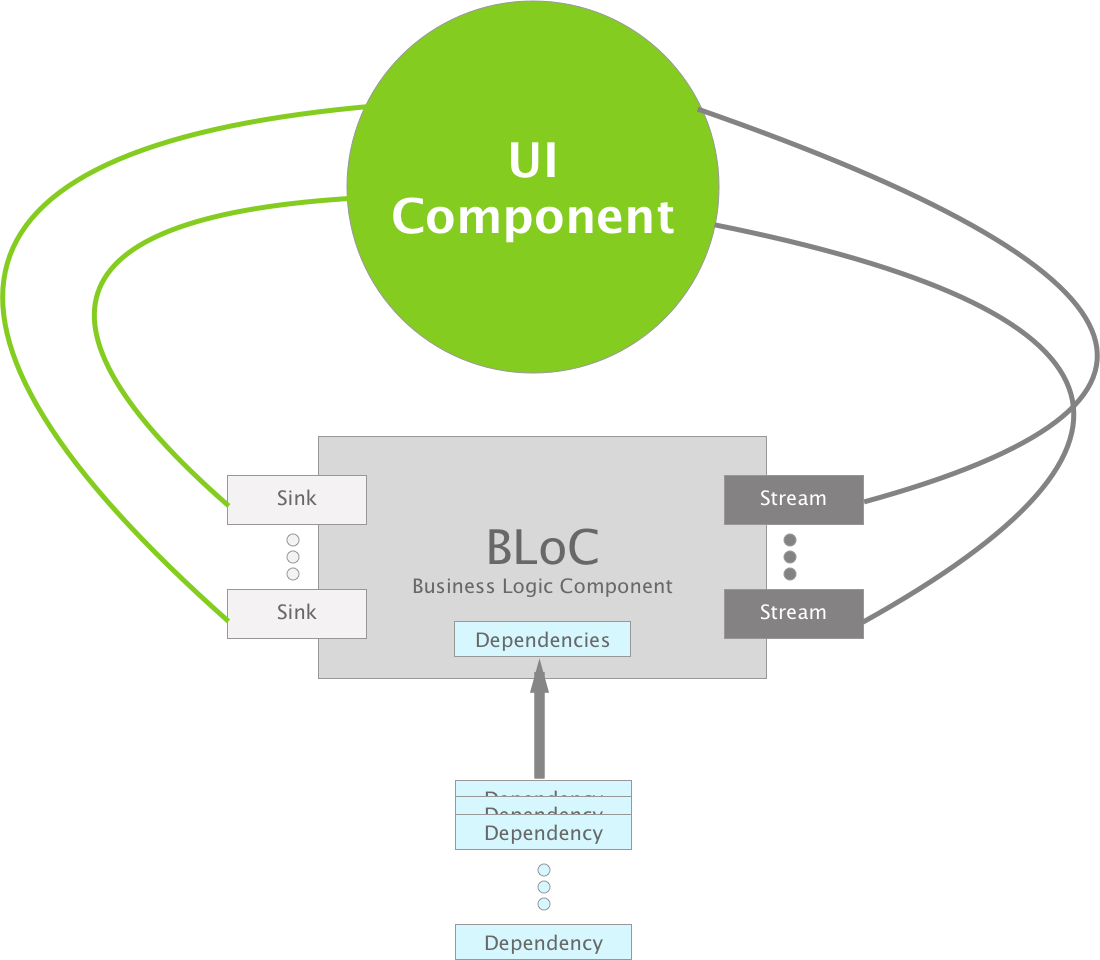
\includegraphics[width=0.8\textwidth]{figures/BLoCPattern.png}
    \caption{A illustration of the BLoC Pattern}
    \label{fig:blocPattern}
\end{figure}

The \gls{bloc} pattern can be boiled down to a set of rules and one practice. The practice is that the business and UI logic should be clearly seperated, where all the business logic should live inside a specific \gls{bloc}. An application should have multiple \gls{bloc}, deciding how to divide the business logic into multiple \glspl{bloc} is a judgement call as Paolo Soares puts it "each complex enough component has its own BLoC" \cite[24 min 15 sec]{blocPattern}. The rules of the \gls{bloc} pattern are listed in \autoref{subsubsec: Bloc_design_guidelines} and \autoref{UI_design_guidelines} as presented by Paolo Soares \cite[22 min 25 sec]{blocPattern}.

\subsubsection{BLoC Design Guidelines} \label{subsubsec: Bloc_design_guidelines}
\begin{itemize}
  \item Inputs and outputs are simple Streams/Sinks only
  \item Dependencies must be injectable and platform agnostic
  \item No platform branching allowed
  \item Implementation can be whatever you want if you follow the previous rules
\end{itemize}

The first rule states that any communication between the \gls{ui} and a \gls{bloc} must be through Sinks or Streams, so when the \gls{ui} should send data to the \gls{bloc} it should be a sink, and when a \gls{bloc} should send data to the \gls{ui} it should be a stream.

The second rule states that all dependency of a \gls{bloc} must be injectable; this is a crucial step in reaching platform independence and does not require much explanation.

The third rule states that one is not allowed to branch depending on the platform, meaning the business logic should be completely independent of the platform. What the rule is effectively stating is that inside a \gls{bloc} there should not be e.x., an if-statement checking if the platform is iOS and do some computation on behave of that.

The last and fourth rule can be a bit hard to understand, but what it states is that one can implement the \gls{bloc} pattern however they like, i.e., like in the Giraf Project using rxDart and thereby reactive programming.

\subsubsection{UI Design Guidelines} \label{subsubsec: UI_design_guidelines}
\begin{itemize}
  \item Each "Complex enough" component has a corresponding \gls{bloc}
  \item Components should send inputs "as is"
  \item Components should show outputs as close as possible to "as is"
  \item All branching should be based on simple \gls{bloc} Boolean outputs
\end{itemize}

The first rule states that if the \gls{ui} component is complex enough it should have its own \gls{bloc}, thereby also stating that \gls{ui} components should share \glspl{bloc} if they are non-complex.

The second rule states that if the \gls{ui} needs to send data to the \gls{bloc}, i.e., User inputs, the \gls{ui} component is not allowed to do any computation on the inputs before sending it to the \gls{bloc}; this is a step to ensure decoupling between the \gls{ui} and Business logic.

The third rule is the same as the second rule but in the other direction. So the output from a \gls{bloc} should not be changed inside the \gls{ui} component, this again is to ensure that all business logic stays inside the \gls{bloc}.

The fourth rule states that all if statements inside the \gls{ui} component should only depend on one boolean stream from the \gls{bloc}, this again is to decouple the \gls{ui} component from the business logic, since branching in the \gls{ui} most likely are based on some business logic.

\subsection{BLoC Implementation in the Giraf Project}
As mentioned the \gls{bloc} pattern is used in the Giraf Project, a number of considerations where taken in implementing the pattern. The first considerations where why should we use the \gls{bloc} pattern. This was chosen since the flutter framework is not opinionated towards one architecture over another, therefore a clear architecture needs to be declared for the development, a number of different patterns where researched including the MVVM and MVC. To better judge the useability of a pattern a set of goals where discussed, the point being that the pattern of chose should reach as many goals as possible. The goals where:

\begin{itemize}
  \item Business logic should be re-useable by all widgets
  \item There should be a clear seperation between \gls{ui} and business logic.
  \item \gls{ui} components should be reactively, ie. if data changes in one component then the change should automaticly be reflected in all other components relying on the same data.
  \item The pattern should allow for a intuitive file structure.
\end{itemize}

Doing some empirical experiments in building with the different patterns and reading different developers experience with the different patterns we came to the conclusion that the \gls{bloc} pattern offered the most freedom while still isolating the business logic and \gls{ui} logic. The \gls{bloc} pattern also allow for all the other goals. This discovery in combination with the fact we only had 3 days to complete the rebuild, we decided on using the \gls{bloc} pattern.

When implementing the \gls{bloc} pattern, some reasearch went into discovering how experienced developers did it, remember that the rules of \gls{bloc} pattern states that it can be implemented in any way you like. When looking at the community around the \gls{bloc} pattern inside flutter it became clear that rxDart was a community favorite library for \gls{bloc} implementation. Therefore we decided to follow the community, since we believe it allow for easier development since there exists many great resources on how to use it and also it will most likely not be aboneded any time soon.

\subsubsection{What is rxDart}
"RxDart is a reactive functional programming library for Google Dart, based on ReactiveX." \cite{rxDart}. It utilizes the native stream support of the Dart Language, to add the missing functionalities of ReactiveX \cite{rxDart}. To better understand how it helps in implementing the \gls{bloc} pattern we will provide a short explanation of what ReactiveX is and describe the key features from the rxDart library that are used in the Giraf Project.

ReactiveX is a library in which one can use observable sequences to create asynchronous and event-based programs, "It extends the observer pattern to support sequences of data and/or events and adds operators that allow you to compose sequences together declaratively while abstracting away concerns about things like low-level threading, synchronization, thread-safety, concurrent data structures, and non-blocking I/O." \cite{ReactiveXWebsite}.

The main features used from the rxDart library are three different stream behaviours, which are PublishSubject, BehaviorSubject and ReplaySubject.

\subsubsection*{PublishSubject}
\begin{figure}[h]
    \centering
    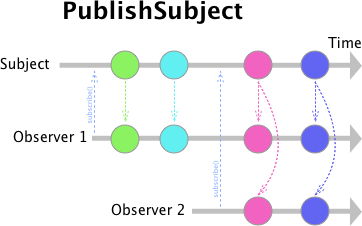
\includegraphics[width=0.8\textwidth]{figures/PublishSubject.png}
    \caption{A illustration of the behavior of a PublishSubject}
    \label{fig:PublishSubject}
\end{figure}
The PublishSubject behaves like the Dart Lang native StreamController, but with one exception, which is that a PublishSubject returns a Observable, where a StreamController returns a stream \cite{PublishSubject}. This means that the PublishSubject upholds the ReactiveX Subject contract and there by allow for all the ReactiveX operations \cite{PublishSubject}. The behaviour of a PublishSubject across time is shown in \autoref{fig:PublishSubject}.

\subsubsection*{BehaviorSubject}
\begin{figure}[h]
    \centering
    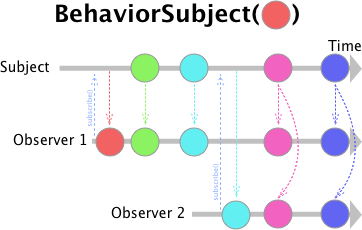
\includegraphics[width=0.8\textwidth]{figures/BehaviorSubject.png}
    \caption{A illustration of the behavior of a BehaviorSubject}
    \label{fig:BehaviorSubject}
\end{figure}
The BehaviorSubject behaves similar to the PublishSubject, but with one exception, it captures the latest item that has been added to the subject and emits that as the first item every time a new observer subscribes \cite{BehaviorSubject}. The BehaviorSubject can also be seeded with a initial item, that will be the first item emitted incase no items has been added to the subject yet. The behaviour of a BehaviorSubject across time is shown in \autoref{fig:BehaviorSubject}.

\subsubsection*{ReplaySubject}
\begin{figure}[h]
    \centering
    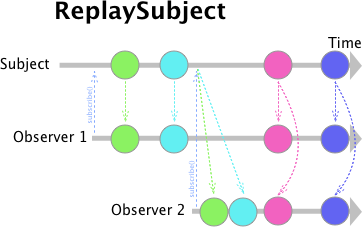
\includegraphics[width=0.8\textwidth]{figures/ReplaySubject.png}
    \caption{A illustration of the behavior of a ReplaySubject}
    \label{fig:ReplaySubject}
\end{figure}
The ReplaySubject behaves similar to the BehaviorSubject, but instead of only capturing the latest item, it captures all items and emits them when ever a new observer subscribes \cite{ReplaySubject}. Unlike the BehaviorSubject, the ReplaySubject can not be seeded with an initial value. The behaviour of a ReplaySubject across time is shown in \autoref{fig:ReplaySubject}
%Firstly the Giraf Project do not have any other platform than the mobile-applications that should utilize the \glspl{bloc} therefore we chose to ignore the rule that all inputs should be sinks, instead we decided that inputs should either be function-calls or sinks. This was to allow developers with limited experience in asynchronous programming to have a easier learning curve.

\subsection{BLoC Design Guidelines of the Giraf Project}
As mentioned earlier the Giraf Project have altered the rules of the \gls{bloc} pattern a bit. The reason for this is that in the Giraf Project we are not using the code in other platforms than the Flutter Framework, therefore to make the use of \glspl{bloc} a bit more intuitive and flexible for the developers we have constructed the following design guideline:

\subsubsection{Giraf Project BLoC Pattern Guidelines}
\begin{itemize}
  \item Rather many small non-complex \glspl{bloc} than few large complex \glspl{bloc}
  \item Start by creating a \gls{bloc} per \gls{ui} Screen, then after implementing the functionality consider to refactor to shared \glspl{bloc}
  \item Inputs to \glspl{bloc} should be either Sinks or function calls with parameters
  \item \glspl{bloc} should be instantiated via the dependency injector/ Thereby all dependencies should also be injectable
  \item \glspl{bloc} are to be implemented using the rxDart library
\end{itemize}


